%\documentclass[wcp,gray]{jmlr} % test grayscale version
 %\documentclass[wcp]{jmlr}% former name JMLR W\&CP
\documentclass[pmlr]{jmlr}% new name PMLR (Proceedings of Machine Learning)

 % The following packages will be automatically loaded:
 % amsmath, amssymb, natbib, graphicx, url, algorithm2e

 %\usepackage{rotating}% for sideways figures and tables
\usepackage{longtable}% for long tables

 % The booktabs package is used by this sample document
 % (it provides \toprule, \midrule and \bottomrule).
 % Remove the next line if you don't require it.
\usepackage{booktabs}
 % The siunitx package is used by this sample document
 % to align numbers in a column by their decimal point.
 % Remove the next line if you don't require it.
\usepackage[load-configurations=version-1]{siunitx} % newer version
 %\usepackage{siunitx}

\makeatletter
\def\set@curr@file#1{\def\@curr@file{#1}} %temp workaround for 2019 latex release
\makeatother

 % The following command is just for this sample document:
\newcommand{\cs}[1]{\texttt{\char`\\#1}}

 % Define an unnumbered theorem just for this sample document:
\theorembodyfont{\upshape}
\theoremheaderfont{\scshape}
\theorempostheader{:}
\theoremsep{\newline}
\newtheorem*{note}{Note}

 % change the arguments, as appropriate, in the following:
\jmlrvolume{}
\jmlryear{2020}
\jmlrworkshop{Machine Learning for Healthcare}

% Short headings should be running head and authors last names
% \ShortHeadings{A Really Awesome MLHC Article}{Lastname, PhD and Lastname, MD}
% \firstpageno{1}

\title[Short Title]{Comparisons Between Hamiltonian Monte Carlo and Maximum A Posteriori For A Bayesian Model For Apixaban Induction Dose \& Dose Personalization}

\author{\Name{A. Demetri Pananos}
       \Email{apananos@uwo.ca}\\ 
       \addr Department of Epidemiology and Biostatistics\\
       Western University\\
		London, Ontario, Canada
       \AND
       \Name{Daniel J. Lizotte}
       \Email{dlizotte@uwo.ca}\\ 
       \addr Department of Epidemiology and Biostatistics\\
       Department of Computer Science\\
       Western University\\
       London, Ontario, Canada} 

\editor{Editor's name}

%My imports
\usepackage{cleveref}
\begin{document}

\maketitle

\begin{abstract}
Precision medicine’s slogan is “right drug -- right patient -- right time”, which is implicitly preceded by “right dose”. However, determining the right dose for any one patient can be challenging because existing models for dose personalization require more data than can reasonably be obtained in order to truly personalize doses.  Bayesian methods, with their ability to explicitly pass prior information to the model, have been proposed as a solution to this problem. Hamiltonian Monte Carlo (HMC) is largely considered the gold standard for fitting Bayesian models, and yet several dose personalization studies use Maximum A Posteriori (MAP) methods to fit their models.  In this study, we put forth a new Bayesian pharmacokinetic model for apixaban pharmacokinetics written in an open source Bayesian language.  We make the model code and posterior summaries of all parameters publicly available. We also perform a simulation study characterizing the differences between inferences made via MAP and HMC for personalized dosing strategies. We find that the differences between HMC and MAP are non-trivial and can greatly affect the choices surrounding dose selection for personalized medicine.

\end{abstract}

%I like to break apart the sections in this way so that editing and debugging is not
% a complete cluster fuck as it usually is in LaTeX
\section{Introduction}

Precision medicine’s slogan is ``right drug -- right patient -- right time''.  Implicit in the slogan is ``right dose''; however, determining the right dose for any one patient can be challenging. The anticoagulant Warfarin offers a good example of these challenges; physicians choose an initial dose based on guidelines and their own experience. They then closely monitor the patient’s International Normalised Ratio (INR), which measures how long it takes blood to clot, and in response they adjust the dose over time.

Pharmacokinetic and statistical models of how drugs behave within an individual can alleviate some of these challenges by predicting the effects of different doses based on patient covariates. In some studies \citep{schwarz2008genetic,Sohrabi2017-zv, Caldwell2007-mi}  a cohort of patients will have an appropriate maintenance doses determined empirically and these are then regressed onto patient covariates.  In others \citep{ohara2019differences,Zhu2017-rk, Xue2017-mp}  patient pharmacokinetics are directly modeled and can be simulated under different dosing regimens to find an appropriate dose.  In both cases, uncertainty in the models can be assessed and can help guide clinical decisions as to what dose is best or what dose to try next.

Both types of  models can provide guidance for individual patients, but only when there is enough data so that the models are accurate and reliable. For personalized pharmacokinetics-based dosing, this amount of data is rarely available in practice.  Obtaining sufficient data to learn a patient’s pharmacokinetic parameters requires a lengthy observation period which few patients are willing or capable of committing to. Population pharmacokinetic models could be used in place of a patient’s pharmacokinetics, but treating the patient as “average” is precisely what precision medicine seeks to improve upon.

In many contexts where limited data area available, Bayesian methods with informative priors have been proposed.  Model priors allow analysts to specify their beliefs about model parameters prior to seeing a new patient's data, and to combine those beliefs with new observations to form personalized predictive models.  This allows models to ``hit the ground running'' so to speak, and makes use of all available data to support decision-making.  To use all but the simplest of Bayesian models for decision-making requires computational approximation techniques to obtain model estimates and predictions. Several approaches exist for generating approximate samples from the posterior distribution, with Hamiltonian Monte Carlo (HMC) being considered the gold standard \citep{Neal1996-vn, Matthew_D_Hoffman2014-in, Carpenter2017-qf, Tripuraneni2017-oh}. Despite HMC being the preferred method by theorists and applied Bayesians alike, methods like Maximum A Posteriori (MAP), in which the posterior mode is computed via optimization and then a Laplace approximation is performed, continue to be used in population Bayesian pharmacokinetic studies as late as 2020 \citep{Brooks2016-li, Nguyen2016-pg,  Preijers2019-kc,Stifft2020-uq}. HMC and MAP are two different approaches with different strengths and different theoretical motivations. Naturally, this raises questions regarding how decisions in personalized medicine may be affected by the use of different methods for performing inference, even using the same model and data. We seek to answer these questions by developing a new, high-fidelity Bayesian pharmacokinetic model and then investigating the impact of the choice of inference method on precision medicine decisions. 

\subsection*{Generalizable Insights about Machine Learning in the Context of Healthcare}

The main methodological insight we gained was that \textit{although predictions made by HMC and MAP may appear to be very similar according to common error metrics, they can lead to very different personalized dosing decisions.} The main contributions of this paper are as follows: 

\begin{enumerate}
\item A new Bayesian model for apixaban pharmacokinetics written in an open source Bayesian language.  We make the model code and posterior summaries of all parameters publicly available at \href{https://github.com/Dpananos/PKBayes}{https://github.com/Dpananos/PKBayes}.

\item A simulation study demonstrating that inferences made via MAP and HMC lead to very different dosing strategies.

\item An induction dosing model for apixaban based on desired trough concentration level after a first dose.
\end{enumerate}





\section{Background}
\subsection*{Pharmacokinetic Modelling}

Broadly, pharmacokinetics is the study of the dynamics of a mass of drug in the body and is concerned with the absorption, distribution, metabolism, and excretion of that drug.  Differential equations (equations which relate the derivative of an unknown function to itself) are often used to describe how these dynamics evolve over time. The differential equation models in pharmacokinetics are called “compartmental models” as they idealize different parts of the body as compartments from which drug can flow in and out at rates proportional to how much drug is presently in that compartment. If the differential equation is not too complex, the solution can be written in terms of analytic functions.  In the case where the differential equation can not be solved in terms of analytic functions, a rich literature of numerical techniques exist to approximate the solution to within quantifiable precision. In either case, estimation of model parameters is of  interest as they represent pharmacokinetic measures, such as the volume of distribution or rate constants for which the drug is absorbed into/excreted out of a compartment. If the parameters for such a model are known, we can use the models to make predictions about drug concentration as a function of time and dose. This in turn can be used to select a dose that meets given criteria about what the concentration function should look like.

Parameter estimation for these models can be done in both frequentist and Bayesian frameworks.  In a Bayesian framework, parameter estimation begins by specifying a prior distribution which reflects the knowledge of parameters before seeing data. Once data are observed, Bayes’ rule can be used to get the posterior distribution.  This distribution provides information about what parameter values have most plausibly generated the observed data.  By virtue of being a probability distribution, the posterior can be summarized by expectations to get point estimates of model parameters. Shown in \cref{fig:fig1} is a visual summary of how Bayes’ rule and Bayesian modelling of pharmacokinetics works using pseudodata. The leftmost panel is our prior distribution.  Each concentration curve results from specific combinations of parameters for the model which are believed to be plausible before seeing data.  Once data are observed (the middle panel), application of Bayes’ rule yields the rightmost panel.  Concentration curves in this panel correspond to combinations of parameters which have most plausibly generated the data, resulting in concentration curves which have most plausibly generated the data. Note that in this setting, because we have many measurements, the pharmacokinetic model is well-determined and the posterior uncertainty is small. Except in very simple cases, the integrals required to evaluate the posterior quickly become intractable, thus computational approximations are required to fit Bayesian models.
%
\begin{figure} [h!]
	\centering
	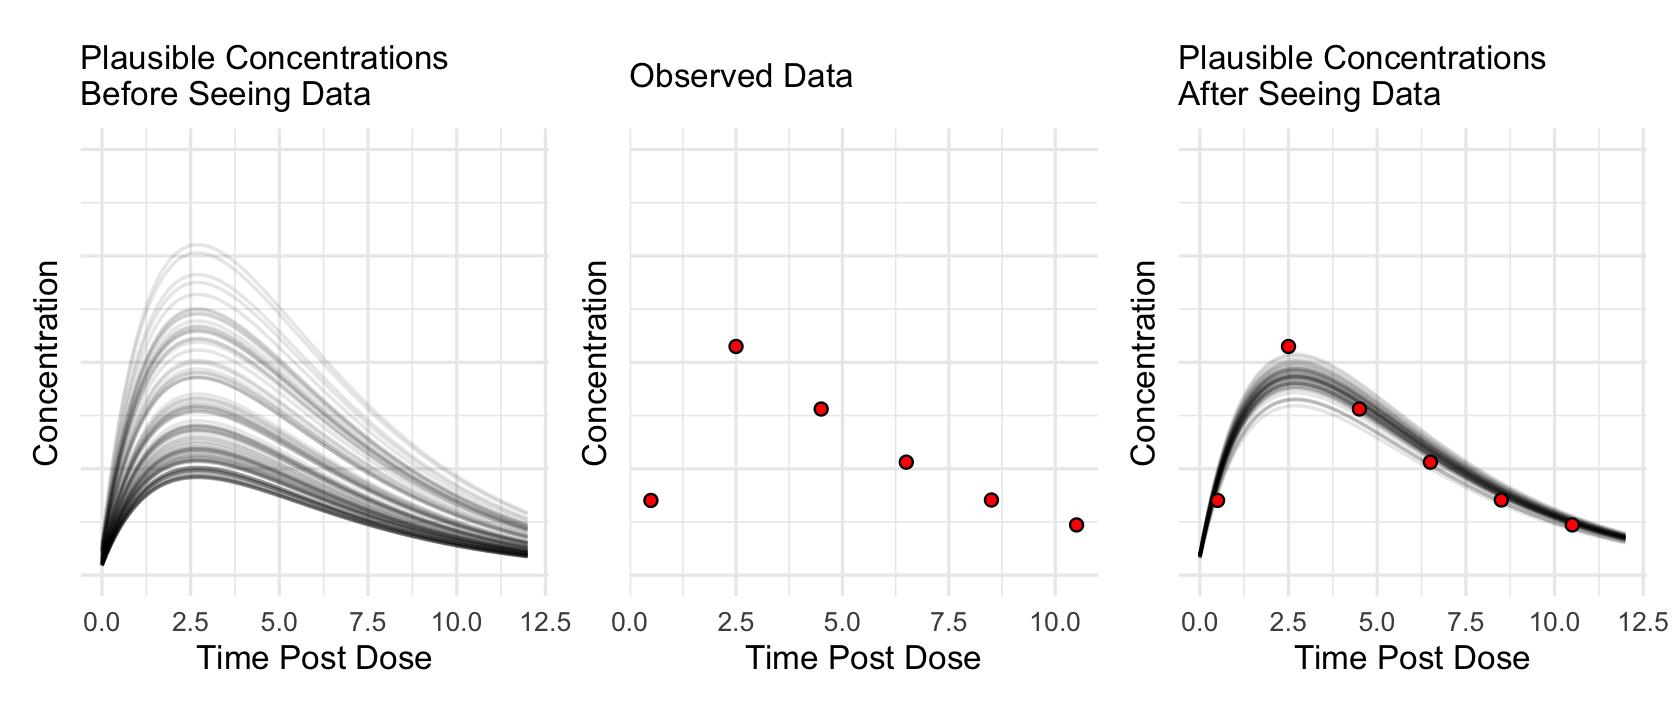
\includegraphics[width=\linewidth]{figs/fig_1}
	\caption{A demonstration of a Bayesian workflow for pharmacokientic models.  The leftmost panel represents the prior.  Each curve corresponds to a unique set of model parameters which induce each concentration function.  In the center panel is the data observed from a single patient.  Conditioning on this data yields the rightmost panel.  Each curve corresponds to a unique set of model parameters drawn from the posterior distribution.} 
	\label{fig:fig1}
\end{figure}
%
\subsection*{Dosing Decisions}

Vitamin K antagonists, such as the popular oral anticoagulant Warfarin, are known to have narrow therapeutic windows as well as drug and food interaction. Determination of a maintenance dose is consequently a procedure with frequent monitoring and followup, with some sources recommending monitoring daily or every other day until the INR stabilizes for two days.  The narrow therapeutic window forces investigators to also consider the pharmacodynamics (the study of the onset, intensity, and duration of the drug response and how these are related to the concentration of the drug at its site of action) of Warfarin in addition with the pharmacokinetics when determining dose size as concentration of the drug alone is not sufficient to infer the antithrombotic effect in patients. The introduction of factor Xa inhibitors like apixaban has alleviated some of the difficulties in prescribing anticoagulants.  Factor Xa inhibitors have been shown to have lower risk for bleeding than Warfarin in patients with atrial fibrillation \cite{vinogradova2018risks} and also allow for fixed dosing without frequent monitoring INR. Furthermore, unlike Warfarin, the pharmacodynamic effect of apixaban on clotting is closely correlated with the concentration in the plasma \cite{Byon2019-gf}, making pharmacokinetic modelling more informative on antithrombotic effect as compared to Warfarin.  However, as of writing this paper there is little information on the therapeutic window, making selecting dose sizes large enough to avoid thromboembolism difficult. Furthermore, studies have demonstrated that inter-patient variability of apixaban plasma concentrations is much higher than was initially believed {\bf CITE MARKUS}. In this work, we develop personalized dosing whose goal is to find the minimum dose that avoids plasma concentrations that are too low. 


\bibliography{references}



\end{document}
